\subsection{Induction}
\hrulefill

\paragraph*{Definition}
Induction is the process of generating an electromotive force in a closed circuit by changing the magnetic field around the circuit.
It is the basis of many electrical devices, including transformers and generators. Induction is governed by Faraday's Law of Induction,
which states that the induced electromotive force in a circuit is equal to the negative rate of change of the magnetic flux through 
the circuit. This is given by the following equations:

\begin{align*}
    \varepsilon &= -\frac{d\Phi_B}{dt} = -\frac{\Delta \Phi_B}{\Delta t}\\
    \varepsilon &= -N\frac{d\Phi_B}{dt} = -N\frac{\Delta \Phi_B}{\Delta t}\\
    \varepsilon &= \frac{d}{dt}(BA\cos(\theta)) = -BA\sin(\theta)
\end{align*}

Where $\varepsilon$ is the electromotive force in volts, $N$ is the number of turns in the coil, $\Phi_B$ is the magnetic flux in webers,
$B$ is the magnetic field in teslas, $A$ is the area of the coil in square meters, and $\theta$ is the angle between the magnetic field
and the normal to the coil.\\

\paragraph*{Lenz's Law}
Lenz's Law states that the direction of the induced current in a circuit is such that it opposes the change in magnetic flux that caused it. 
Practically, this means that when the magnetic flux increases, an opposing magnetic field is generated to counteract the increase. 
Conversely, if the magnetic flux decreases, the generated magnetic field will be in the same direction as the original field, opposing the 
decrease. The direction of this opposing field determines the direction of the induced current.

\begin{center}
    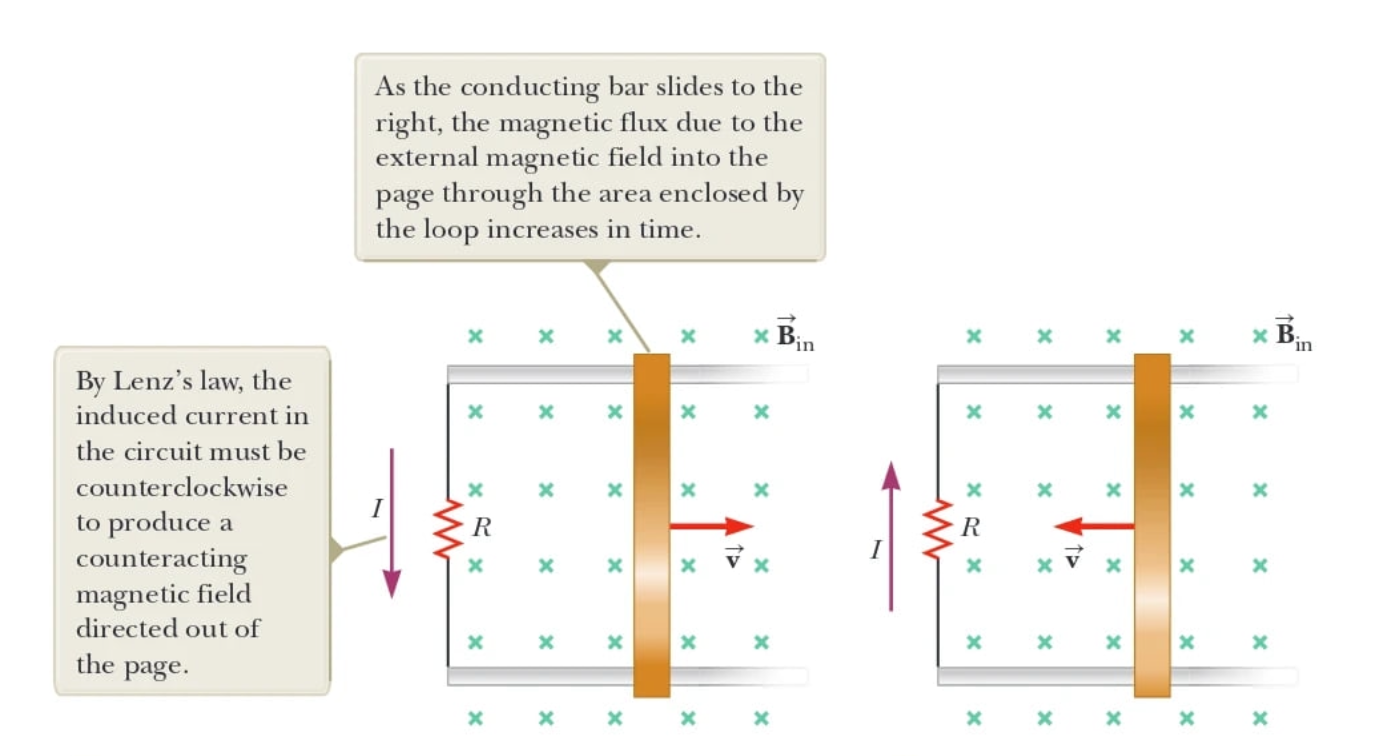
\includegraphics[scale=0.5]{lenz_law.png}
\end{center}